\subsection{Ownable}
"Ownable"-klassen er en abstrakt klasse, der indeholder de atributter, som de felter spillerne kan eje. Klassen er abstrakt, da det ikke skal være muligt at oprette objekter af denne type. Istedet skal de felter der nedarver fra denne klasse oprettes. Klasserne Property, Brewery og Shipping, nedarver alle fra denne klasse. Klassen Ownable indeholder en konstruktør, der tager imod parametrene: title, value, mortgage value og color.
Klassen nedarver fra Field (se figur \ref{fig:fieldArv}) da de felter der kan ejes er en undergruppe af felterne, de har dog stadig nogle fælles attributter som de felter der ikke kan ejes..
\begin{figure}[H]
    \centering
    \includegraphics[width=10cm]{sources/7_implementering/OwnableKonstruktør.PNG}
    \caption{Attributer og konstruktør i Ownable klassen}
    \label{fig:OwnableKons}
\end{figure}
Alle disse paramterer går igen i alle felter der kan ejes. Derudover er atributten Owner af typen "Player" blevet implementeret med en Getter og Setter metode. Dvs sige at hvert felt ved hvem det bliver ejet af. 

\newpage
De 3 felter der er mulige at eje er:

\begin{itemize}
    \item Property
    \item Brewery
    \item Shipping
\end{itemize}

\subsubsection{Property}
Property-feltet udgør hoveddelen af brættet. Der er dem spillerne kan købe, bygge huse og hoteller og modtage leje fra andre spillere. Klassen indeholder et integer array, hvori lejen for 0, 1, 2, 3, 4 og et hotel er gemt. Derudover holder klassen også styr på hvor mange huse og hoteller som er blevet bygget på grunden. Metoden getRent er implementere for at kunne beregne lejen som en spiller, der lander på feltet skal betale. Lejen afhænger af hvor mange huse eller hoteller der er på grunden, og i hvilken farve gruppe grunden er i.

\begin{figure}[H]
    \centering
    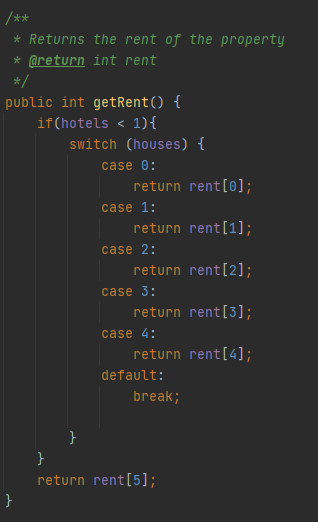
\includegraphics[width=7cm]{sources/7_implementering/propRent.PNG}
    \caption{getRent metoden i Property klassen}
    \label{fig:getRentPR}
\end{figure}

\newpage
\subsubsection{Brewery}
Brewery felterne kan også ejes af spillere. Her kan dog ikke bygges huse eller hoteller. Lejen er beregnet udfra hvad den spiller, der lander på feltet har slået med terningerne og om en spiller ejer begge Brewery felterne i spillet. 

\begin{figure}[H]
    \centering
    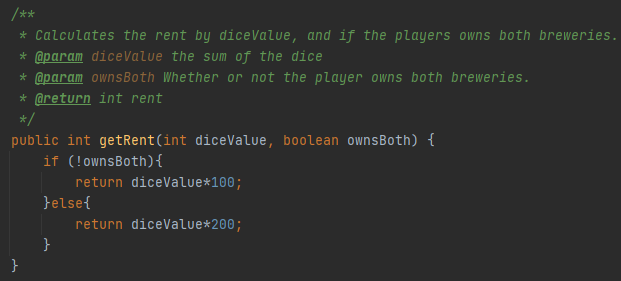
\includegraphics[width=\textwidth]{sources/7_implementering/breweryrent.PNG}
    \caption{getRent metoden i Brewery klassen}
    \label{fig:getRentBR}
\end{figure}

\subsubsection{Shipping}
Det er også muligt for spilleren at eje Shipping felterne. Her kan dog ligesom Brewery feltet, ikke bygges huse eller hoteller. Lejen på Shipping felterne afhænger af hvor mange Shipping felter den pågældende ejer også ejer på brættet. f.eks. hvis ejeren, ejer 1 rederi er lejen 500 kr. Men ejes der 4 rederier er lejen på 4.000 kr. (Se figur \ref{fig:shippingRent}).
\begin{figure}[H]
    \centering
    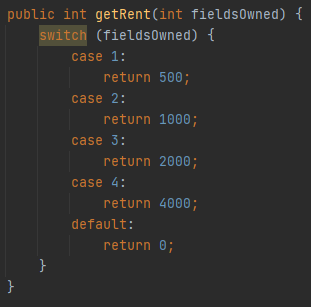
\includegraphics{sources/7_implementering/shippingrent.PNG}
    \caption{getRent metode i Shipping klassen}
    \label{fig:shippingRent}
\end{figure}